\documentclass[a4paper,12pt]{article} % This defines the style of your paper

\usepackage[top = 2.5cm, bottom = 2.5cm, left = 2.5cm, right = 2.5cm]{geometry} 

\usepackage[T2A]{fontenc}
\usepackage[utf8]{inputenc}
\usepackage[russian]{babel}

\usepackage{multirow} 
\usepackage{booktabs} 

\usepackage{graphicx} 

\usepackage{setspace}
\setlength{\parindent}{0in}

\usepackage{float}

\usepackage{amsmath}

\usepackage{fancyhdr}

\usepackage{pgfplots}
\pgfplotsset{compat=1.9}

\pagestyle{fancy} 

\fancyhf{} 

\lhead{\footnotesize Расчетное задание №15}

\rhead{\footnotesize Николаев Юрий} 

\cfoot{\footnotesize \thepage} 

\begin{document}

\thispagestyle{empty} 

\begin{tabular}{p{15.5cm}} 
НИУ МЭИ \\ А-13а-19  \\ Вариант 13 \\ Николаев Юрий\\
\hline 
\\
\end{tabular} 

\vspace*{0.3cm}

\begin{center} 
	{\Large \bf Расчетное задание №15} 
	\vspace{2mm}
\end{center}  

\vspace{0.4cm}


\section{Задание}
Для функции $y = y(x)$, заданной таблицей своих значений, построить интерполяционные многочлены в форме Лагранжа и Ньютона. Используя их, вычислить приближенное значение функции в точке $\bar x$. 

$$\bar x = 0,22$$

\begin{center}
\begin{tabular}{| c | c | c | c | c |}
\hline
    x & 0 & 1 & 2 & 3 \\ \hline
    y & 1 & 4 & 0 & 1 \\
\hline
\end{tabular}
\end{center}

\section{Решение}

\begin{enumerate}

\item Построим многочлен Лагранжа $L_n(x) = \sum\limits_{i = 0}^n y_i \prod\limits_{\substack{k = 0 \\ k \neq i}}^{n} \frac{(x - x_k)}{(x_i - x_k)}$:

$$L_3(x) = y_0 \frac{(x - x_1)(x - x_2)(x - x_3)}{(x_0 - x_1)(x_0 - x_2)(x_0 - x_3)} + y_1 \frac{(x - x_0)(x - x_2)(x - x_3)}{(x_1 - x_0)(x_1 - x_2)(x_1 - x_3)} + $$
$$+ y_2 \frac{(x - x_0)(x - x_1)(x - x_3)}{(x_2 - x_0)(x_2 - x_1)(x_2 - x_3)} + y_3 \frac{(x - x_0)(x - x_1)(x - x_2)}{(x_3 - x_0)(x_3 - x_1)(x_3 - x_2)} = $$
$$= 1 \cdot \frac{(x - 1)(x - 2)(x - 3)}{(-1)(-2)(-3)} + 4 \cdot \frac{(x)(x - 2)(x - 3)}{(1)(1 - 2)(1 - 3)} + 1 \cdot \frac{(x)(x - 1)(x - 2)}{(3)(3 - 1)(3 - 2)}$$

Получили: $$L_3(x) = 2x^3 - \frac{19}{2}x^2 + \frac{21}{2}x + 1$$

Приближенное значение в точке $\bar x$: $L_3(0,22) \approx \textbf{2,8715}$

\item Построим многочлен Ньютона $P_n(x)$:

Составим диагональную таблицу конечный разностей. Шаг таблицы $h = 1$.

\begin{center}
\begin{tabular}{| c | c | c | c | c |}
\hline
    x_i & y_i & \Delta y & \Delta^2 y & \Delta^3 y \\ \hline
    0 & 1 &  &  & \\ \hline
      &   & 3 &  & \\ \hline
    1 & 4 &  & -7 & \\ \hline
      &  & -4 &  & 12 \\ \hline
    2 & 0 &  & 5 & \\ \hline
      &  & 1 &  & \\ \hline
    3 & 1 &  &  & \\
\hline
\end{tabular}    
\end{center}

$$
P_3(x_0 + ht) = 1 + \frac{3t}{1! \cdot 1} - \frac{7t(t - 1)}{2! \cdot 1^2} + \frac{12t(t - 1)(t - 2)}{3! \cdot 1^3} =
$$

$$
= 1 + 3t - \frac{7}{2}t(t - 1) + 2t(t - 1)(t - 2) = 2t^3 - \frac{19}{2}t^2 + \frac{21}{2}t + 1
$$

В нашем случае $x_0 = 0$, $h = 1$, а так как $\bar x = 0,22$, то $t = 0,22$.

Тогда получаем:

$$P_3(x) = 2x^3 - \frac{19}{2}x^2 + \frac{21}{2}x + 1$$

$$
P_3(\bar x) = 2 \cdot (0,22)^3 - \frac{19}{2} \cdot (0,22)^2 + \frac{21}{2} \cdot (0,22) + 1 = 2,8715
$$

Приближенное значение в точке $\bar x$: $P_3(0,22) \approx \textbf{2,8715}$

\begin{figure}[h]
\center{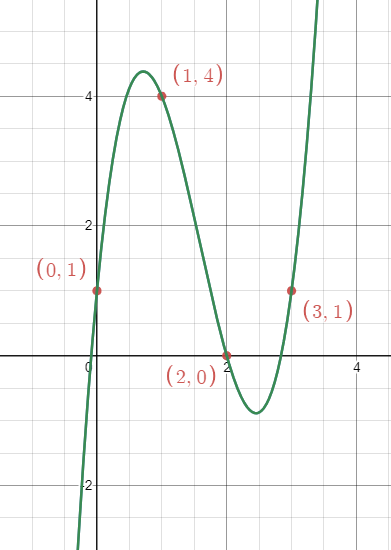
\includegraphics[scale=0.7]{graphic15.png}}
\caption{График исходных точек и многочленов}
\label{fig:image}
\end{figure}

\end{enumerate}

Как мы видим, $L_n(x) = P_n(x)$, отсюда и значения в точке $\bar x$ тоже одинаковые. По графику видно, что функции слились и прошли четко по исходным точкам. 

\end{document}